\section{Regression Results}
Physics based models are used to predict a continuous value for bathymetry.
Regression \ac{ML} models were fit in order to compare to existing models.
Three models were fit to the data: 
an SVM regression model, a Naive Bayes regression model, and a simple linear regression model.
These models were trained against a reduced set of data shown in figure \ref{fig:trainset}, and validated against the rest of the world.

\begin{figure}[h]
    \centering
    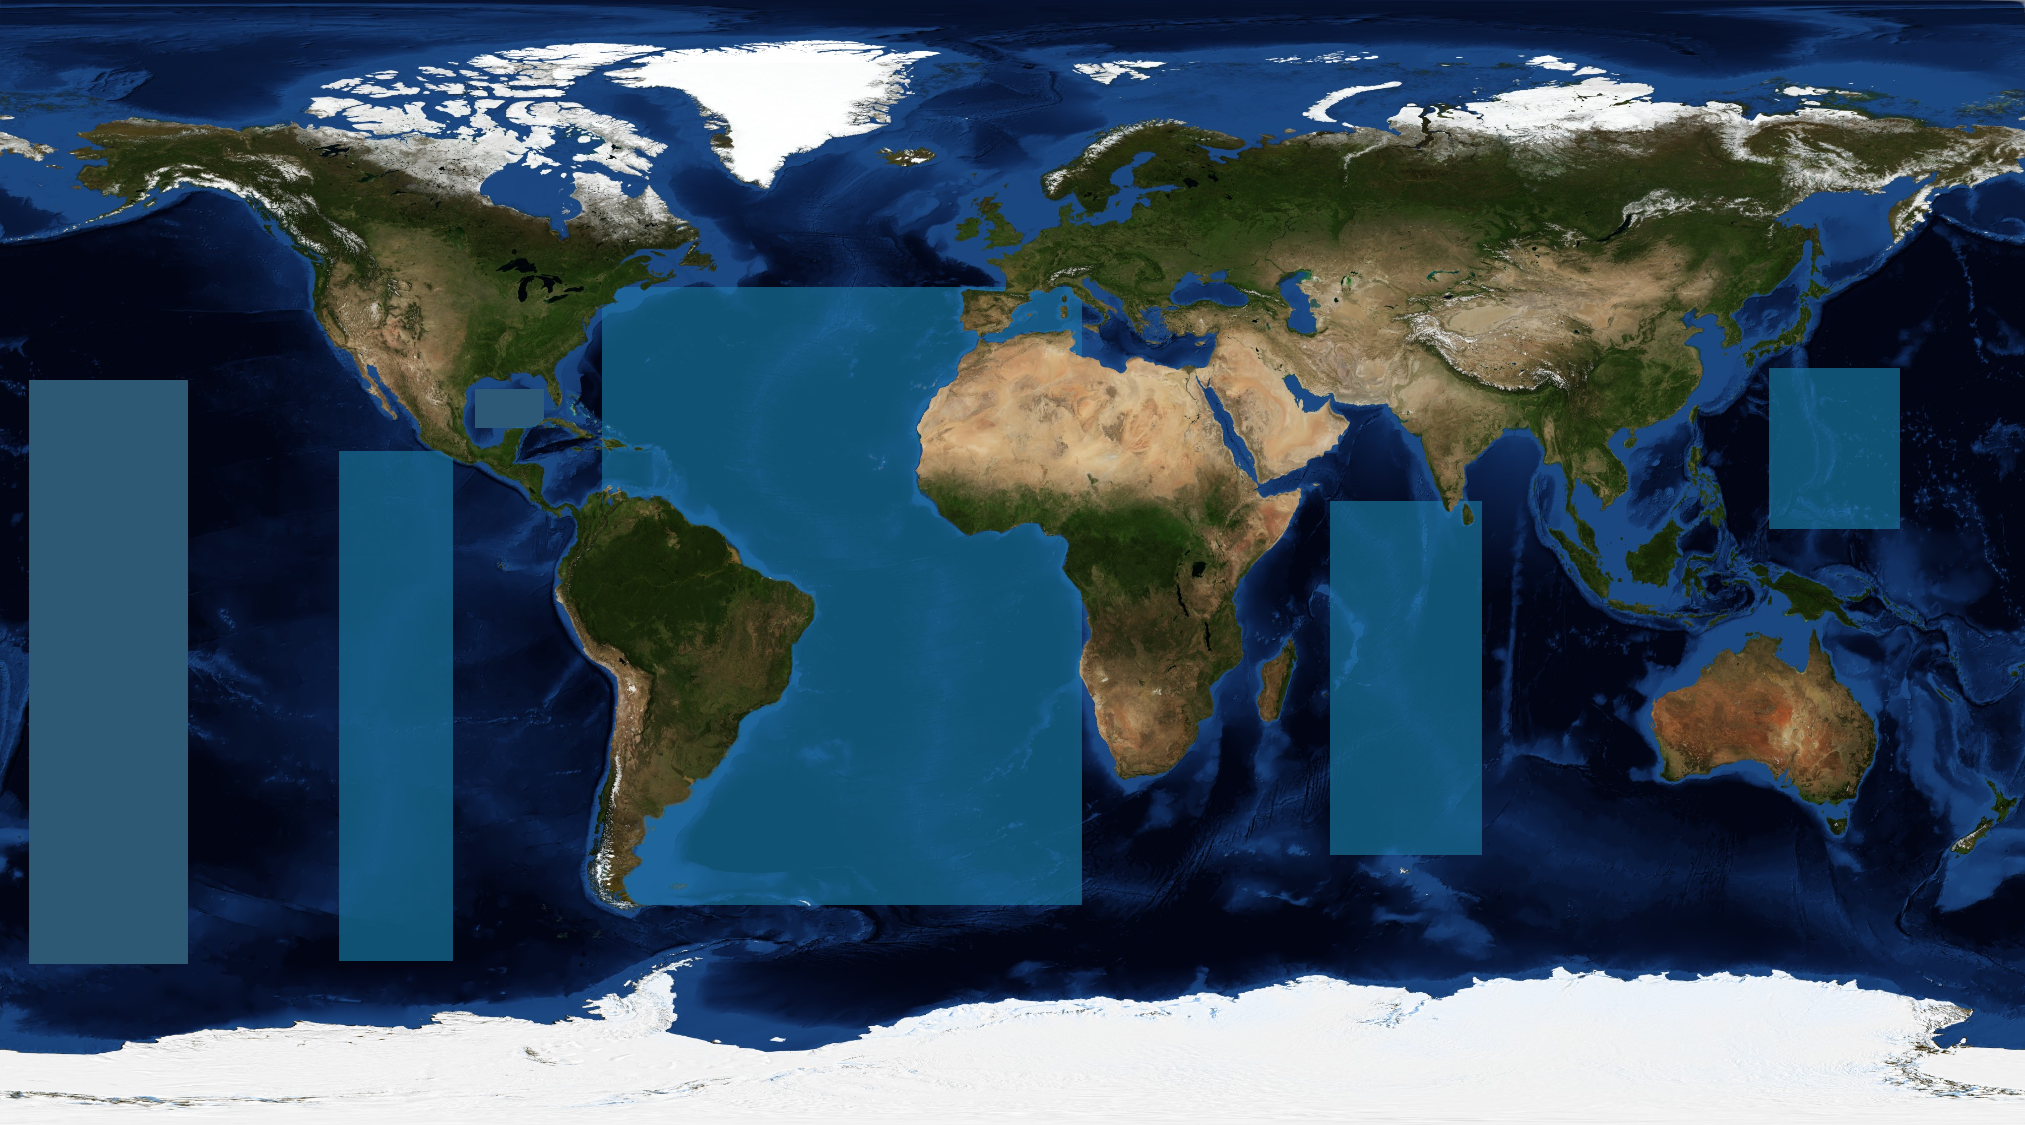
\includegraphics[width=\textwidth]{worldtraininglocal.png}
    \caption{Figure demonstrating initial training sets.}
    \label{fig:trainset}
\end{figure}

\begin{table}[htp]
    \centering
    \begin{tabular}{|c c c|}
        \hline
		\textbf{Model} & \textbf{\(R^2\)} & \textbf{RMSE} \\
		\hline
		SVM Regression & 0.841 & 365.23m \\
		Naive Bayes & 0.884 & 294.92m \\
        Linear Regression & 0.885 & 265.43m \\
	    \hline
    \end{tabular}
    \label{table:REGRESSION_RESULTS}
    \caption{Regression Results}
\end{table}

\subsection{Regression Results Discussion}
\cite{jena2012prediction} achieved a \ac{RMSE} of \~{}175m in their optimized model.
The linear regression model I fit is 100 meters less accurate than the optimized model used in \cite{jena2012prediction}.
However, the purpose of the test is not to achieve accurate predictions, but to identify if \ac{ML} models can be viable.
Therefore, the accuracy of these models is less important than identifying the viability of the models.
The training data used is essentially predicted bathymetry, but shows that fitting a model to true bathymetry will yield a similar result.
Analyzing the \(R^2\) score gives evidence of the viability of the model.
This score suggests that there are underlying relationships in the model that can be used to train a successful model.


%
%
%end{tabular}

% \begin{sidewaysfigure}[h]
%     \centering
%     \begin{tikzpicture}
%         \node[align=left,draw] 
% 		at ([yshift=-35pt]current bounding box.south)
% 		{%
% 			\begin{tabular}{c l c l c l c l}

% 				\begin{tikzpicture}
% 					\draw[fill opacity=0.5,fill=rfc] (0,0) rectangle (1,0.25);
% 				\end{tikzpicture}
% 				& RandonForestClassifier &  

% 				\begin{tikzpicture}
% 					\draw[fill opacity=0.5,fill=ada] (0,0) rectangle (1,0.25);
% 				\end{tikzpicture}
% 				& AdaBoostClassifier &

% 				\begin{tikzpicture}
% 					\draw[fill opacity=0.5,fill=grad] (0,0) rectangle (1,0.25);
% 				\end{tikzpicture}
%                 & GradientBoostingClassifier & 
% 				\begin{tikzpicture}
% 					\draw[fill opacity=0.5,fill=qda] (0,0) rectangle (1,0.25);
% 				\end{tikzpicture}
%                 & QDA \\ 
% 				\begin{tikzpicture}
% 					\draw[fill opacity=0.5,fill=dtc] (0,0) rectangle (1,0.25);
% 				\end{tikzpicture}
%                 & DecisionTree & 
% 				\begin{tikzpicture}
% 					\draw[fill opacity=0.5,fill=voting] (0,0) rectangle (1,0.25);
% 				\end{tikzpicture}
%                 & VotingClassifier & 

% 				\begin{tikzpicture}
% 					\draw[fill opacity=0.5,fill=bag] (0,0) rectangle (1,0.25);
% 				\end{tikzpicture}
%                 & Bagging &                
%                 \begin{tikzpicture}
% 					\draw[fill opacity=0.5,fill=mlp] (0,0) rectangle (1,0.25);
% 				\end{tikzpicture}
%                 & ANN \\
% 				\begin{tikzpicture}
% 					\draw[fill opacity=0.5,fill=knn] (0,0) rectangle (1,0.25);
% 				\end{tikzpicture}
%                 & KNN &

% 				\begin{tikzpicture}
% 					\draw[fill opacity=0.5,fill=gau] (0,0) rectangle (1,0.25);
% 				\end{tikzpicture}
%                 & NaiveBayes &
%                 \begin{tikzpicture}
% 					\draw[fill opacity=0.5,fill=land] (0,0) rectangle (1,0.25);
% 				\end{tikzpicture}
%                 & LAND \\
% 			\end{tabular}
% 		};
%     \end{tikzpicture}
%     \caption{}
%     \label{}
% \end{sidewaysfigure}